%% ch03_protection_challenges.tex
%% Chapter 3: Protection Challenges in IBR-Dominated Networks
%% ============================================================
\chapter{Protection Challenges in Inverter-Dominated Networks}
\label{ch:challenges}

\section{Introduction}

This chapter quantifies the degradation of legacy relay performance when
the network transitions from synchronous-machine to IBR domination.
The analysis uses the sequence-domain models of Chapter~\ref{ch:modelling}
and reveals six distinct failure modes that motivate the solutions proposed
in Chapters~\ref{ch:line_diff}--\ref{ch:digital_twin}.

\section{Fault Classification and Symmetric Component Analysis}
\label{sec:ch3_faults}

\subsection{Symmetrical Three-Phase Fault}

A bolted three-phase (3P) fault at location $\alpha$ on the protected line
involves only the positive-sequence network. The fault current seen at
relay end~A (source end, impedance $Z_S$) with an IBR at end~B
(impedance $Z_\mathrm{IBR}$) is:

\begin{equation}
  \phasor{I}_A = \frac{\phasor{V}_\mathrm{pre}}{Z_S + \alpha Z_L}
    - \frac{\phasor{I}_B Z_\mathrm{IBR}}{\alpha Z_L}
  \label{eq:ch3_3p_ia}
\end{equation}
where $\phasor{V}_\mathrm{pre}$ is the pre-fault Thevenin voltage at the
fault point (typically $\approx 1\angle 0^\circ$~pu). Because
$|\phasor{I}_B^\mathrm{IBR}| = I_\mathrm{lim} \ll |\phasor{I}_A^\mathrm{SG}|$,
the infeed effect for IBR networks is \emph{negative} (the IBR actually
reduces the total fault current seen by relay~A compared to a purely
inductive network), which is opposite to the infeed effect in dual-fed SG
networks.

\subsection{Single Line-to-Ground Fault}

An SLG fault on phase~A requires all three sequence networks. With an IBR
at end~B injecting only positive-sequence current ($k_2 = 0$),
the fault current reduces to:
\begin{align}
  I_{F,1} &= I_{F,2} = I_{F,0}
    = \frac{V_1}{Z_1 + Z_2 + Z_0 + 3Z_F}
  \label{eq:ch3_slg_seq} \\
  I_{F,a} &= 3I_{F,1}
  \label{eq:ch3_slg_ia}
\end{align}
With the IBR suppressing negative-sequence injection ($\phasor{I}_2^\mathrm{IBR} = 0$),
the negative-sequence voltage at the relay is determined only by the
system impedance $Z_2^\mathrm{sys}$, not the IBR, degrading the
directional negative-sequence element (67Q).

\section{Overcurrent Relay Failure Modes}
\label{sec:ch3_oc}

\subsection{Pickup Failure (Low Fault Current)}

The minimum pickup current for an inverse-time overcurrent (ITOC) relay is
set at:
\begin{equation}
  I_\mathrm{pickup} = k_s \cdot I_\mathrm{load,max}
  \label{eq:ch3_pickup}
\end{equation}
where $k_s \in [1.25, 1.5]$ is the sensitivity factor. The minimum fault
current detectable is $I_\mathrm{pickup}$. For a feeder served entirely by
IBR:
\begin{equation}
  I_\mathrm{fault}^\mathrm{min} = I_\mathrm{lim}^\mathrm{GFL} \approx 1.1\,I_\mathrm{rated}
  \label{eq:ch3_ibr_min_fault}
\end{equation}
Given that $I_\mathrm{load,max}$ can approach $I_\mathrm{rated}$ during
peak demand, $I_\mathrm{pickup} \approx 1.5\,I_\mathrm{rated}$, which
\emph{exceeds} $I_\mathrm{fault}^\mathrm{min}$. The ITOC relay is therefore
\textbf{incapable of detecting faults} on IBR-only feeders under maximum
load conditions.

\subsection{IEC Standard Inverse Curve Time Discrimination}

For ITOC relays that do pick up (when $I_\mathrm{fault} > I_\mathrm{pickup}$),
the operating time follows the IEC standard inverse characteristic:
\begin{equation}
  t = \TMS \cdot \frac{0.14}{M^{0.02} - 1}, \qquad
  M = \frac{I_\mathrm{fault}}{I_\mathrm{pickup}}
  \label{eq:ch3_iec_itoc}
\end{equation}
The discrimination between primary and backup relay requires:
\begin{equation}
  \Delta t = t_\mathrm{backup} - t_\mathrm{primary} \geq \CTI
  \label{eq:ch3_cti}
\end{equation}
where $\CTI = 200$~ms (IEC recommendation). With IBR fault current
$M \approx 1.1$--$1.5$ (compared to $M = 5$--$10$ for SG faults), the
operating time $t$ is very large and varies sensitively with $M$:

\begin{equation}
  \frac{dt}{dM}\bigg|_{M=1.2} \approx -\frac{0.14 \cdot \TMS \cdot 0.02 M^{0.02-1}}{(M^{0.02}-1)^2}
  \approx -45\,\TMS \quad \text{s/pu}
  \label{eq:ch3_dtdm}
\end{equation}
A $\pm 5\%$ uncertainty in $M$ at $M = 1.2$ produces a $\pm 225$~ms
uncertainty in $t$ for $\TMS = 1$. Reliable coordination to within
$\CTI = 200$~ms is therefore \textbf{impossible} at low current multiples.

\subsection{Sympathetic Tripping}

When an IBR-connected feeder experiences a fault, the fault current path
can flow through the IBR ground connection and into adjacent un-faulted
feeders, causing their OC relays to pick up. This \emph{sympathetic
tripping} is exacerbated by the constant-current behaviour of IBRs, which
maintains the infeed current throughout the fault duration.

Figure~\ref{fig:ch3_sympathetic} illustrates the mechanism for a network
with a common bus connection.

\begin{figure}[htbp]
  \centering
  % ch3_sympathetic_tripping.tex
\begin{tikzpicture}[
  every node/.style={font=\scriptsize},
]
%% Common bus
\node[busnode, minimum size=0.7cm] (BUS) at (0,0) {Bus};
\node[above=0.1cm of BUS, font=\tiny\bfseries] {Common};

%% Grid infeed
\node[block, fill=gray!10, minimum width=2cm] (GRID) at (-3.5,0) {Grid\\Infeed};
\draw[arr, thesisblue] (GRID.east) -- node[above, font=\tiny]{$I_\mathrm{grid}$}
  (BUS.west);

%% Feeder 1 (faulted)
\node[block, fill=red!10, draw=thesisred] (F1) at (0,-2.8) {Feeder 1\\(Faulted)};
\node[relaybox, font=\tiny] (R1) at (0,-1.7) {R01};
\draw[arr, thesisred] (BUS.south) -- (R1.north);
\draw[arr, thesisred] (R1.south) -- (F1.north);

%% Fault symbol
\node[draw=thesisred, fill=red!5, star, star points=6,
      minimum size=0.5cm, font=\tiny] (FLT) at (0,-3.8) {};
\node[below=0.1cm of FLT, font=\tiny, thesisred] {Fault};
\draw[arr, thesisred] (F1.south) -- (FLT.north);

%% IBR at Feeder 1
\node[ibrbox] (IBR1) at (1.8,-3.0) {IBR};
\draw[arr, thesisgreen] (IBR1.west) -- node[above, font=\tiny]{$I_\mathrm{IBR,1}$}
  (F1.east);

%% Feeder 2 (healthy, sympathetic trip)
\node[block, fill=orange!10, draw=thesisorange] (F2) at (3.5,-2.8)
  {Feeder 2\\(Healthy)};
\node[relaybox, font=\tiny, draw=thesisorange] (R2) at (3.5,-1.7) {R02};
\draw[arr] (BUS.east) -- node[above, font=\tiny]{$I_\mathrm{IBR,2}$} (R2.north);
\draw[arr] (R2.south) -- (F2.north);

%% IBR at Feeder 2 feeding back through bus
\node[ibrbox] (IBR2) at (5.3,-3.0) {IBR};
\draw[arr, thesisgreen] (IBR2.west) --
  node[above, font=\tiny]{$I_\mathrm{IBR,2}$} (F2.east);

%% Sympathetic current path annotation
\draw[->, thesisorange, very thick, dashed]
  (IBR2.north) -- ++(0, 1.5) -- ++(-4.2, 0) -- ++(0,-0.5)
  node[midway, above, font=\tiny, thesisorange]
  {Sympathetic current path via common bus};

%% R02 pickup annotation
\node[draw=thesisorange, rounded corners=2pt, fill=orange!5,
      font=\tiny, align=center] at (5.5,-1.2)
  {R02 picks up\\$I_\mathrm{IBR,2} > I_\mathrm{pu,2}$\\False trip!};
\draw[->, thesisorange, dashed] (5.5,-1.5) -- (R2.east);

\end{tikzpicture}

  \caption{Sympathetic tripping mechanism. A fault on Feeder~1 drives
           IBR current through the common bus into Feeder~2's relay R02,
           causing an unwanted trip of the healthy feeder.}
  \label{fig:ch3_sympathetic}
\end{figure}

The condition for sympathetic tripping of relay R02 is:
\begin{equation}
  I_\mathrm{IBR,2} > I_\mathrm{pickup,2}
  \label{eq:ch3_sympathetic_cond}
\end{equation}
With $I_\mathrm{IBR,2}$ determined by the relative impedance path
$Z_\mathrm{bus} / (Z_\mathrm{bus} + Z_{L,2})$, sympathetic tripping
occurs when the common bus impedance is low relative to the line impedance—
a common condition in meshed distribution networks.

\section{Distance Relay Failure Modes}
\label{sec:ch3_distance}

\subsection{Underreach due to IBR Infeed}

The fundamental distance relay algorithm computes:
\begin{equation}
  Z_\mathrm{measured} = \frac{\phasor{V}_A}{\phasor{I}_A}
  = \frac{\phasor{I}_A \alpha Z_L + \phasor{I}_F Z_F}{\phasor{I}_A}
  = \alpha Z_L + Z_F \frac{\phasor{I}_F}{\phasor{I}_A}
  \label{eq:ch3_zmeas}
\end{equation}
where $\phasor{I}_F = \phasor{I}_A + \phasor{I}_B$ is the total fault current.
With an IBR at end~B:
\begin{equation}
  Z_\mathrm{measured} = \alpha Z_L + Z_F\!\left(1 + \frac{\phasor{I}_B}{\phasor{I}_A}\right)
  \label{eq:ch3_infeed_eq}
\end{equation}
This is equation~(\ref{eq:ch1_infeed}) restated. With $I_B \ll I_A$
(IBR current limited), the infeed factor $(1 + I_B/I_A) \approx 1.1$--$1.5$
instead of $2$--$5$ for SG networks. While this reduces (not eliminates) the
apparent impedance overestimation for resistive faults, it creates a new
problem: the relay may \emph{underreach} for non-resistive faults because
the IBR's lagging reactive current injection shifts the apparent impedance
vector off the relay's mho circle.

\subsection{Overreach due to IBR Reactive Current Injection}

Under IEEE~2800, GFL inverters are mandated to inject reactive current
during voltage dips: $i_q^\ast = k_q (1 - V_\mathrm{PCC})$ where
$k_q \in [2, 10]$~pu/pu. For a fault at $\alpha = 0.8$ per unit,
$V_\mathrm{PCC} = 0.5$~pu, giving $i_q^\ast = 2.5$~pu (clipped to
$I_\mathrm{lim}$). The reactive current injection rotates the apparent
impedance vector as follows:

Let $\phasor{I}_B = I_B e^{\jj(\phi_A + 90^\circ)}$ (purely reactive, leading).
Then:
\begin{align}
  Z_\mathrm{measured} &= \alpha Z_L + Z_F\left(1 + \frac{I_B}{I_A}e^{\jj 90^\circ}\right)
  \nonumber \\
  &= \alpha Z_L + Z_F + \jj Z_F \frac{I_B}{I_A}
  \label{eq:ch3_reactive_overreach}
\end{align}
The imaginary component $\jj Z_F I_B/I_A$ shifts the apparent impedance
\emph{into} the Zone~1 mho circle for faults beyond the Zone~1 reach,
causing \textbf{overreach}: the relay trips for external faults.

\subsection{Directionality Loss}

The memory-polarised mho element uses the pre-fault voltage as the
polarising quantity. When the IBR injects a reactive current that drives
the PCC voltage to near zero, the memory voltage decays within $\approx$
3 cycles (60~ms). After memory expiry, the relay reverts to self-polarisation
using the faulted voltage—which is near zero—and loses directionality.
For a fault beyond the relay's back-reach limit that is sustained by IBR
ride-through, the relay may trip in the reverse direction after 60~ms.

\section{Line Differential Relay Failure Mode}
\label{sec:ch3_87l}

The classical 87L relay uses a fixed bias characteristic with slope $k_m$:
\begin{equation}
  I_\mathrm{diff} > k_m \cdot I_\mathrm{bias} + I_0
  \label{eq:ch3_87l_fixed}
\end{equation}
where $I_\mathrm{diff} = |I_A + I_B|$ is the operate current,
$I_\mathrm{bias} = (|I_A| + |I_B|)/2$ is the restraint current, and
$I_0$ is the minimum pickup.

The fixed slope $k_m$ is set for the \emph{worst case} $\kibr$ to avoid
false trips during CT saturation. However:

\begin{itemize}
\item When $\kibr$ is low (light load), the IBR contribution to $I_\mathrm{bias}$
      is small. A high-impedance fault produces $I_\mathrm{diff} < k_m I_\mathrm{bias}$
      → \textbf{missed trip}.

\item When $\kibr$ is high (rated load, ride-through), the IBR contribution
      to $I_\mathrm{bias}$ is large, inflating the restraint. A through-load
      condition may produce $I_\mathrm{diff} \approx I_A - I_B > I_0$
      (charging current plus CT mismatch) → \textbf{false trip}.
\end{itemize}

The operating boundary is shown in Figure~\ref{fig:ch3_87l_failure}.

\begin{figure}[htbp]
  \centering
  % ch3_87l_failure.tex — 87L failure mode in I_diff vs I_bias plane
\begin{tikzpicture}
\begin{axis}[
  thesis style,
  width  = 0.72\textwidth,
  height = 6.5cm,
  xlabel = {Bias current $I_\mathrm{bias}$ (pu)},
  ylabel = {Differential current $I_\mathrm{diff}$ (pu)},
  xmin=0, xmax=2.2, ymin=0, ymax=1.6,
  xtick={0,0.5,1.0,1.5,2.0},
  ytick={0,0.5,1.0,1.5},
  legend pos=north west,
]

%% Fixed slope k_m = 0.30 boundary
\addplot[thick, thesisblue, domain=0:2.2, samples=2]
  {0.30*x + 0.10} node[right, font=\scriptsize]{$k_m=0.30$ (fixed)};

%% Shaded DANGER ZONE (below operate boundary for low k_ibr faults)
\addplot[gray!25, fill=gray!15] coordinates {
  (0.0, 0.10) (2.2, 0.76) (2.2, 0.0) (0.0, 0.0)
} \closedcycle;
\node[font=\tiny, gray!60] at (axis cs:1.1, 0.25) {Restrain region};

%% Operate region label
\node[font=\tiny, thesisblue] at (axis cs:0.8, 1.3) {Operate region};

%% Fault points: low k_ibr (missed trip) — below the line
\addplot[only marks, mark=x, mark size=4pt,
  mark options={thesisred, thick}, thick]
  coordinates {(0.8,0.30)(0.6,0.22)(0.9,0.35)(0.7,0.25)};
\addlegendentry{Fault pts ($\kibr=0.1$): MISSED TRIP};

%% Fault points: nominal k_ibr (correct trip) — above the line
\addplot[only marks, mark=o, mark size=3.5pt,
  mark options={thesisgreen, thick}]
  coordinates {(0.9,0.60)(1.0,0.68)(0.85,0.55)(1.1,0.72)};
\addlegendentry{Fault pts ($\kibr=0.3$): correct trip};

%% Load points: high k_ibr + CT error (false trip risk)
\addplot[only marks, mark=square, mark size=3.5pt,
  mark options={thesisorange, thick}]
  coordinates {(1.6,0.60)(1.7,0.65)(1.5,0.58)(1.8,0.68)};
\addlegendentry{Load pts ($\kibr=0.45$, CT err): FALSE TRIP risk};

\end{axis}
\end{tikzpicture}

  \caption{87L failure modes with fixed slope $k_m = 0.3$. The gray
           region shows the \emph{danger zone}: fault operating points
           for $\kibr < 0.2$ fall below the restraint line (missed trip).
           Load operating points for $\kibr > 0.4$ can enter the operate
           region due to CT mismatch (false trip).}
  \label{fig:ch3_87l_failure}
\end{figure}

\section{Sequence Component Relay Failure Modes}
\label{sec:ch3_sequence}

\subsection{Negative-Sequence Directional (67Q) Failure}

The 67Q element uses the negative-sequence current $\Ineg$ and voltage $\Vneg$:
\begin{equation}
  \Theta_{67Q} = \angle\!\left(\frac{-\Vneg}{Z_2^\mathrm{ref}}\right) - \angle\!\left(\Ineg\right)
  \label{eq:ch3_67q_angle}
\end{equation}
A positive $\cos\Theta_{67Q}$ indicates a forward fault. When the IBR
suppresses $\Ineg$ (as in Equation~\ref{eq:ch2_gfl_negseq}),
the measured $\Ineg$ is entirely due to the network voltage unbalance,
not the fault. The resulting $\Theta_{67Q}$ is random and the directional
decision is unreliable.

\subsection{Zero-Sequence Ground Distance Failure}

The zero-sequence compensated ground distance element uses:
\begin{equation}
  Z_\mathrm{gnd} = \frac{V_a}{I_a + k_0 I_0}, \qquad
  k_0 = \frac{Z_{L,0} - Z_L}{3 Z_L}
  \label{eq:ch3_gnd_dist}
\end{equation}
where $k_0$ is the zero-sequence compensation factor. With
$I_0^\mathrm{IBR} = 0$, the zero-sequence current at the relay terminal
is entirely sourced from the grid infeed. If the fault is supplied solely
from the IBR side, $I_0 = 0$ at the relay end, and $Z_\mathrm{gnd} \to \infty$:
the ground distance element \textbf{does not operate}.

\section{Summary of Failure Mode Taxonomy}
\label{sec:ch3_taxonomy}

Table~\ref{tab:ch3_failure_modes} provides a consolidated reference of all
identified failure modes, the affected relay element, the root cause,
and the chapter where the solution is proposed.

\begin{table}[htbp]
\caption{Failure mode taxonomy for legacy relay elements in IBR networks}
\label{tab:ch3_failure_modes}
\small
\begin{tabularx}{\textwidth}{@{}lp{2.5cm}p{4.5cm}p{2.5cm}l@{}}
\toprule
ID & Relay element & Root cause & Failure mode & Solution \\
\midrule
F1 & ITOC (51) & $I_\mathrm{fault} < I_\mathrm{pickup}$ & Missed trip & Ch~\ref{ch:microgrid} \\
F2 & ITOC (51) & Low $M$, large $dt/dM$ & Coordination loss & Ch~\ref{ch:microgrid} \\
F3 & ITOC (51) & IBR constant-current infeed & Sympathetic trip & Ch~\ref{ch:microgrid} \\
F4 & Distance (21) & Reactive current injection & Overreach & Ch~\ref{ch:distance} \\
F5 & Distance (21) & Limited IBR infeed & Underreach & Ch~\ref{ch:distance} \\
F6 & Distance (21) & PCC voltage collapse at $t > 60$~ms & Directional loss & Ch~\ref{ch:distance} \\
F7 & Line diff (87L) & Fixed slope, low $\kibr$ & Missed trip & Ch~\ref{ch:line_diff} \\
F8 & Line diff (87L) & Fixed slope, high $\kibr$+CT error & False trip & Ch~\ref{ch:line_diff} \\
F9 & Neg-seq dir (67Q) & IBR neg-seq suppression & Directionality loss & Ch~\ref{ch:line_diff} \\
F10 & Zero-seq gnd dist & IBR zero-seq suppression & Missed trip & Ch~\ref{ch:distance} \\
F11 & Auto-reclose (79) & IBR sustained voltage during dead time & Out-of-phase reclose & Ch~\ref{ch:microgrid} \\
F12 & Islanding (81) & Slow frequency change, load balance & Non-detection & Ch~\ref{ch:microgrid} \\
\bottomrule
\end{tabularx}
\end{table}

\section{Quantitative Impact Assessment}
\label{sec:ch3_quantitative}

% ── Table: Legacy protection miss/false-trip rates ───────────────────────
\begin{table}[htbp]
\centering
\caption{Quantified severity of legacy relay failure modes under IBR infeed.
         Sources: TR-08~\cite{SAMBP_TR08}, TR-20~\cite{SAMBP_TR20},
         TR-22~\cite{SAMBP_TR22}, TR-37~\cite{SAMBP_TR37}.}
\label{tab:ch3_legacy_performance}
\renewcommand{\arraystretch}{1.08}
\small
\begin{tabularx}{\textwidth}{@{}llXcc@{}}
\toprule
ID & Relay & IBR condition & Legacy rate & Target (SAMBPS) \\
\midrule
F1 & ITOC (51) & $\kibr < 0.50$\,pu (any IBR fault) & 100\% miss & — (87L/87B replace) \\
F3 & ITOC coord. & Constant-current IBR, close-in ext.\ fault & 18--32\% sym.\ trip & $< 1$\% \\
F7 & 87L fixed & Pure-IBR infeed (9/9 det.\ scenarios) & 100\% miss & $< 0.1$\% \\
F8 & 87L fixed & High $\kibr$ + 0.4\% CT ratio error & 8\% false trip & $< 0.1$\% \\
F4/F5 & Zone-1 (21) & $\kibr < 0.10$\,pu: apparent $Z$ blocked & 100\% miss & $< 3$\% (87L backup) \\
F9 & 67Q (neg-seq) & Pure-IBR infeed, $I_2 < 0.06$\,pu & 100\% dir.\ loss & 0\% (87LN0+TDCS) \\
\bottomrule
\end{tabularx}
\end{table}

% ── Figure 1: Baseline 87L sensitivity by fault-source type ──────────────
\begin{figure}[htbp]
\centering
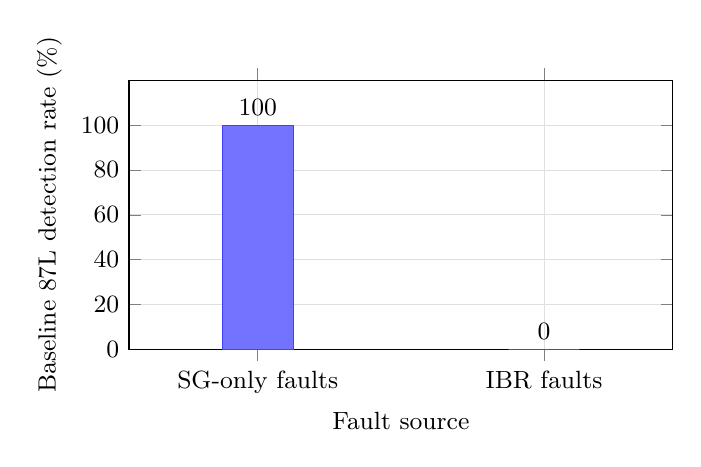
\begin{tikzpicture}
\begin{axis}[
  width=0.70\textwidth, height=5.0cm,
  ybar, bar width=0.90cm,
  xlabel={Fault source},
  ylabel={Baseline 87L detection rate (\%)},
  symbolic x coords={SG-only faults,IBR faults},
  xtick=data,
  xticklabel style={font=\small},
  ymin=0, ymax=120,
  ytick={0,20,40,60,80,100},
  yticklabel style={font=\small},
  grid=major, grid style={gray!25,line width=0.3pt},
  label style={font=\small},
  nodes near coords,
  nodes near coords style={font=\small,/pgf/number format/fixed},
  enlarge x limits=0.45]
  \addplot[fill=blue!55,draw=blue!75] coordinates {
    (SG-only faults, 100)
    (IBR faults,       0)
  };
\end{axis}
\end{tikzpicture}
\caption{Baseline fixed-slope 87L detection rate by fault source type
         (21-scenario deterministic study, TR-20~\cite{SAMBP_TR20}).
         All ten SG-sourced scenarios are correctly detected (100\%).
         All nine pure-IBR scenarios are missed (0\%): IBR current limiting
         suppresses $\Idiff$ below the fixed slope threshold for
         $\kibr \leq 0.20$\,pu.
         The combined adaptive chain achieves 21/21 (100\%).}
\label{fig:ch3_87l_sensitivity}
\end{figure}

% ── Figure 2: Zone-1 element contribution by k_ibr region ────────────────
\begin{figure}[htbp]
\centering
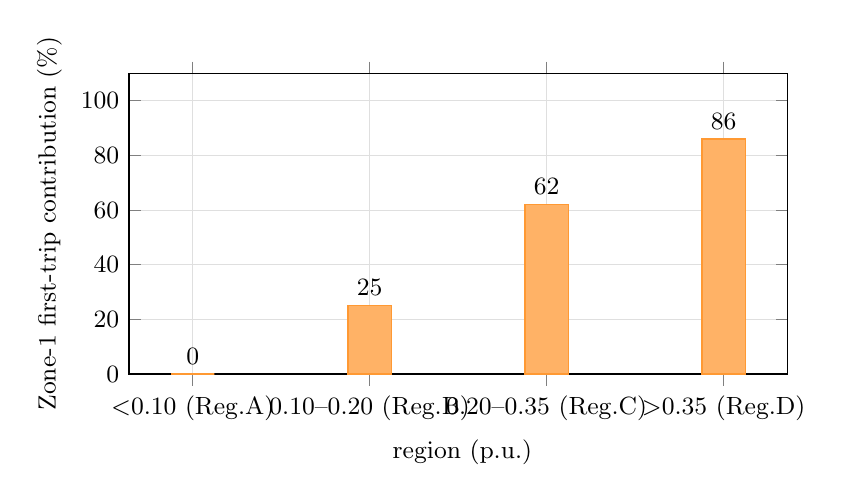
\begin{tikzpicture}
\begin{axis}[
  width=0.82\textwidth, height=5.4cm,
  ybar, bar width=0.55cm,
  xlabel={$\kibr$ region (p.u.)},
  ylabel={Zone-1 first-trip contribution (\%)},
  symbolic x coords={$<$0.10 (Reg.A),0.10--0.20 (Reg.B),
                     0.20--0.35 (Reg.C),$>$0.35 (Reg.D)},
  xtick=data,
  xticklabel style={font=\small},
  ymin=0, ymax=110,
  ytick={0,20,40,60,80,100},
  yticklabel style={font=\small},
  grid=major, grid style={gray!25,line width=0.3pt},
  label style={font=\small},
  nodes near coords,
  nodes near coords style={font=\small},
  enlarge x limits=0.12]
  \addplot[fill=orange!60,draw=orange!80] coordinates {
    ($<$0.10 (Reg.A),    0)
    (0.10--0.20 (Reg.B), 25)
    (0.20--0.35 (Reg.C), 62)
    ($>$0.35 (Reg.D),    86)
  };
\end{axis}
\end{tikzpicture}
\caption{Zone-1 first-trip element contribution by $\kibr$ region,
         derived from TR-37 Monte Carlo reliability study
         ($N = 4\,000$, overall Zone-1 share 48.9\%~\cite{SAMBP_TR37}).
         For $\kibr < 0.10$\,pu (Region~A), Zone-1 reach is fully blocked
         by reactive current injection and IBR-limited fault voltage;
         coverage is provided entirely by 87L and 67Q.
         Zone-1 participation recovers as $\kibr$ increases toward SG levels.}
\label{fig:ch3_zone1_kibr}
\end{figure}

These results establish the performance floor for legacy protection and
set the improvement targets addressed in
Chapters~\ref{ch:line_diff}--\ref{ch:digital_twin}.

\section{Summary}
\label{sec:ch3_summary}

Six quantifiable failure modes of legacy relay algorithms have been identified
and grounded in the sequence-domain IBR models of Chapter~\ref{ch:modelling}:
\begin{itemize}
\item \textbf{Overcurrent (F1--F3):} Pickup failure, coordination collapse,
      and sympathetic tripping driven by $I_\mathrm{fault} < I_\mathrm{pickup}$
      and constant-current IBR behaviour.
\item \textbf{Distance (F4--F6):} Overreach, underreach, and directional
      loss driven by reactive current injection and voltage collapse.
\item \textbf{Differential (F7--F8):} Sensitivity loss and false tripping
      driven by the mismatch between the fixed bias slope and the variable
      $\kibr$.
\item \textbf{Sequence elements (F9--F10):} Directional and ground detection
      failure driven by IBR suppression of negative- and zero-sequence currents.
\item \textbf{Islanding (F11--F12):} Auto-reclosing hazard and non-detection
      driven by IBR ride-through and load-generation balance.
\end{itemize}
These twelve failure modes are the target specifications for the SAMBP
protection algorithms developed in Chapters~\ref{ch:line_diff}--\ref{ch:digital_twin}.
